\subsection*{Method of characteristics}
A scalar hyperbolic conservation is a PDE that can be written in the form 
\begin{equation}
    u_t + \diff f(u) \nabla u = 0,
    \label{eq:general-hyp-cons}
\end{equation}
where $f=(f_1,\dots, f_m)$ and $x=(x_1, \dots, x_n)$\cite{MR3443431}. This can not be done for \eqref{eq:model1-pde} which defines our model in the two-dimensional case because the curvature term is parabolic. However, in the one-dimensional case the curvature reduces to
\begin{equation*}
    \nabla \cdot \frac{\nabla u}{|\nabla u|} = \bigg( \frac{u_x}{|u_x|} \bigg)_x = (\pm 1)_x = 0.
\end{equation*}
We immediately get that \eqref{eq:model1-pde} turns into
\begin{equation*}
    u_t = \pm u_x \alpha \sigma(x) d(x; \pointsetm),
\end{equation*}
which for a $\diff f(u) = \mp \alpha \sigma d(x; \pointsetm)$ is a hyperbolic conservation law as in \eqref{eq:general-hyp-cons}. Because the curvature term is meaningless in one dimensions, this is less interesting seen as it is a key feature for our model. 

In a radially symmetric situation, the curvature is more interesting. The setup is the same as in the calculations leading up to \eqref{eq:J-rad} an is shown in \figref{fig:stationary-example}. For both \pointset\ and $\Gamma$ being circles with the same center, the distance $d(r; \pointsetm) = |r-r_v|$ and the curvature of a circle is known as
\begin{equation}
    \kappa(r) = \frac{1}{r}
    \label{eq:curvature-circle}
\end{equation}
\begin{comment}
\subsection{1 spatial dimension}
\begin{figure}
    \centering
    \includegraphics{figures/tikz-figures/characteristics-1d-initial.tex}
    \caption[Method of characteristics - initial function]{Caption}
    \label{fig:1d-char}
\end{figure}

We look at our equation \todo{ref} in one dimensions. The situation is as pictured in \figref{fig:1d-char}, with the point set consisting of two points, $\mathcal{V}=\{v_1, v_2\}$. We can then assume without loss of generality that they are placed symmetric around the origin. First of all, we notice that in one dimensions, the notion of curvature is meaningless.
\begin{equation}
    \kappa(u) = \Bigg( \frac{u_x}{|u_x|} \Bigg)_x = (\pm 1)_x = 0
\end{equation}

We then have that our level set equation simply is
\begin{equation}
    u_t =\alpha \sigma (x) d(x)\, u_x
\end{equation}

Because our problem is symmetric, the function, $\sigma (x) = \pm 1$, depending on our initial function has a level set that is inside or outside the point set. 

\end{comment}
The term $|\nabla u|$ can be expressed in terms of $r$ through a simple change of variables:
\begin{align*}
    r &=\sqrt{x^2+y^2} \\
    \implies \frac{dr}{dx} &= \frac{x}{\sqrt{x^2 + y^2}} \\
    \implies \frac{dr}{dy} &= \frac{y}{\sqrt{x^2+ y^2}} \\
    |\nabla u| &= \sqrt{u_x^2 + u_y^2} = \sqrt{\frac{\partial u}{\partial r} \frac{dr}{dx} + \frac{\partial u}{\partial r} \frac{dr}{dy}}
\end{align*}
\begin{equation}
    \implies |\nabla u | = \sqrt{\frac{u_r^2}{x^2+y^2} (x^2 + y^2)} = u_r, \qquad \text{if } u_r\geq 0
    \label{eq:nablau-ur}
\end{equation}

Inserting \eqref{eq:curvature-circle} and \eqref{eq:nablau-ur} into \eqref{eq:model1-pde} we get
\begin{equation}
    u_t = u_r \bigg(\alpha \sigma(t)|r-r_v| + \frac{(1-\alpha)}{r} \bigg).
    \label{eq:zero-levelset-polar-coords}
\end{equation}

We have now a conservation law on the form \eqref{eq:general-hyp-cons} for $r$. Because our PDE now is only dependent on the radius, the total derivative of \eqref{eq:zero-levelset-polar-coords} with respect to time becomes
\begin{equation}
    \frac{du}{dt} = u_t + u_r \,r_t.
    \label{eq:polar-characteristic-eq}
\end{equation}

We want to investigate how the curve moves in time. The curve is always the zero level set, and is thus by definition constant and equal to zero. Moreover, the PDE can be even simplified further at the curve because we have that $\sigma(t)(|r_{\Gamma}-r_v|) = (r_{\Gamma}-r_v)$ at the curve, since the sign function changes at the point when $r_{\Gamma}=r_v$. Thus 
\begin{equation}
    u_t = u_r \bigg(\alpha (r-r_v) + \frac{(1-\alpha)}{r} \bigg) \qquad \text{for } r=\radgammam.
    \label{eq:levelset-polar-coords}
\end{equation}
Because of the constant value for $u$ at all level curves, the left hand side in \eqref{eq:polar-characteristic-eq} equals zero. And thus
\begin{equation}
    u_t=-u_r\, r_t,
    \label{eq:characteristic-streamline}
\end{equation}
and by comparing \eqref{eq:characteristic-streamline} with \eqref{eq:zero-levelset-polar-coords}, we see that
\begin{equation}
    r_t = -\bigg(\alpha \sigma|r(t)-r_v| + \frac{(1-\alpha)}{r(t)}\bigg),
    \label{eq:pde-streamline}
\end{equation}
where $r(t)$ is the radius for a single iso-contour which moves in time. We will call the trajectories of the curves following \eqref{eq:pde-streamline}, the streamlines for the solution. First, we want to analyze how the zero level curve moves given an initial radius, $r_0$. We then compare  \eqref{eq:levelset-polar-coords} and \eqref{eq:zero-levelset-polar-coords} to obtain the PDE for the streamline of a zero iso-contour
\begin{equation}
    r_t = -\bigg(\alpha (r(t)-r_v) + \frac{(1-\alpha)}{r(t)}\bigg) \quad \text{for }r(t) = r_{\Gamma}.
    \label{eq:pde-zero-streamline}
\end{equation}

The equation \eqref{eq:pde-zero-streamline} is a separable equation, and the solution is an implicit function of $r(t)$,
\begin{equation}
    \frac{\ln(\alpha(r(t)^2-r_v\,r(t)-1)+1) - \frac{2\sqrt{\alpha}\,r_v \tan^{-1}\bigg(\frac{\sqrt{\alpha} (r_v-2r(t))}{\sqrt{4-\alpha(r_v^2+4)}}\bigg)}{\sqrt{4-\alpha(r_v^2+4)}}}{2\alpha}=-t+C,
    \label{eq:streamline-solution}
\end{equation}
where the constant $C$ is decided from the initial conditions, $t=0$, $r=r_0$.
\begin{equation}
    C=\frac{\ln(\alpha(r_0^2-r_v r_0-1)+1) - \frac{2\sqrt{\alpha}\,r_v \tan^{-1}\bigg(\frac{\sqrt{\alpha} (r_v-2r_0)}{\sqrt{4-\alpha(r_v^2+4)}}\bigg)}{\sqrt{4-\alpha(r_v^2+4)}}}{2\alpha}.
    \label{eq:streamline-solution-constant}
\end{equation}

\begin{figure}
    \begin{subfigure}[b]{0.48\linewidth}
    \centering
        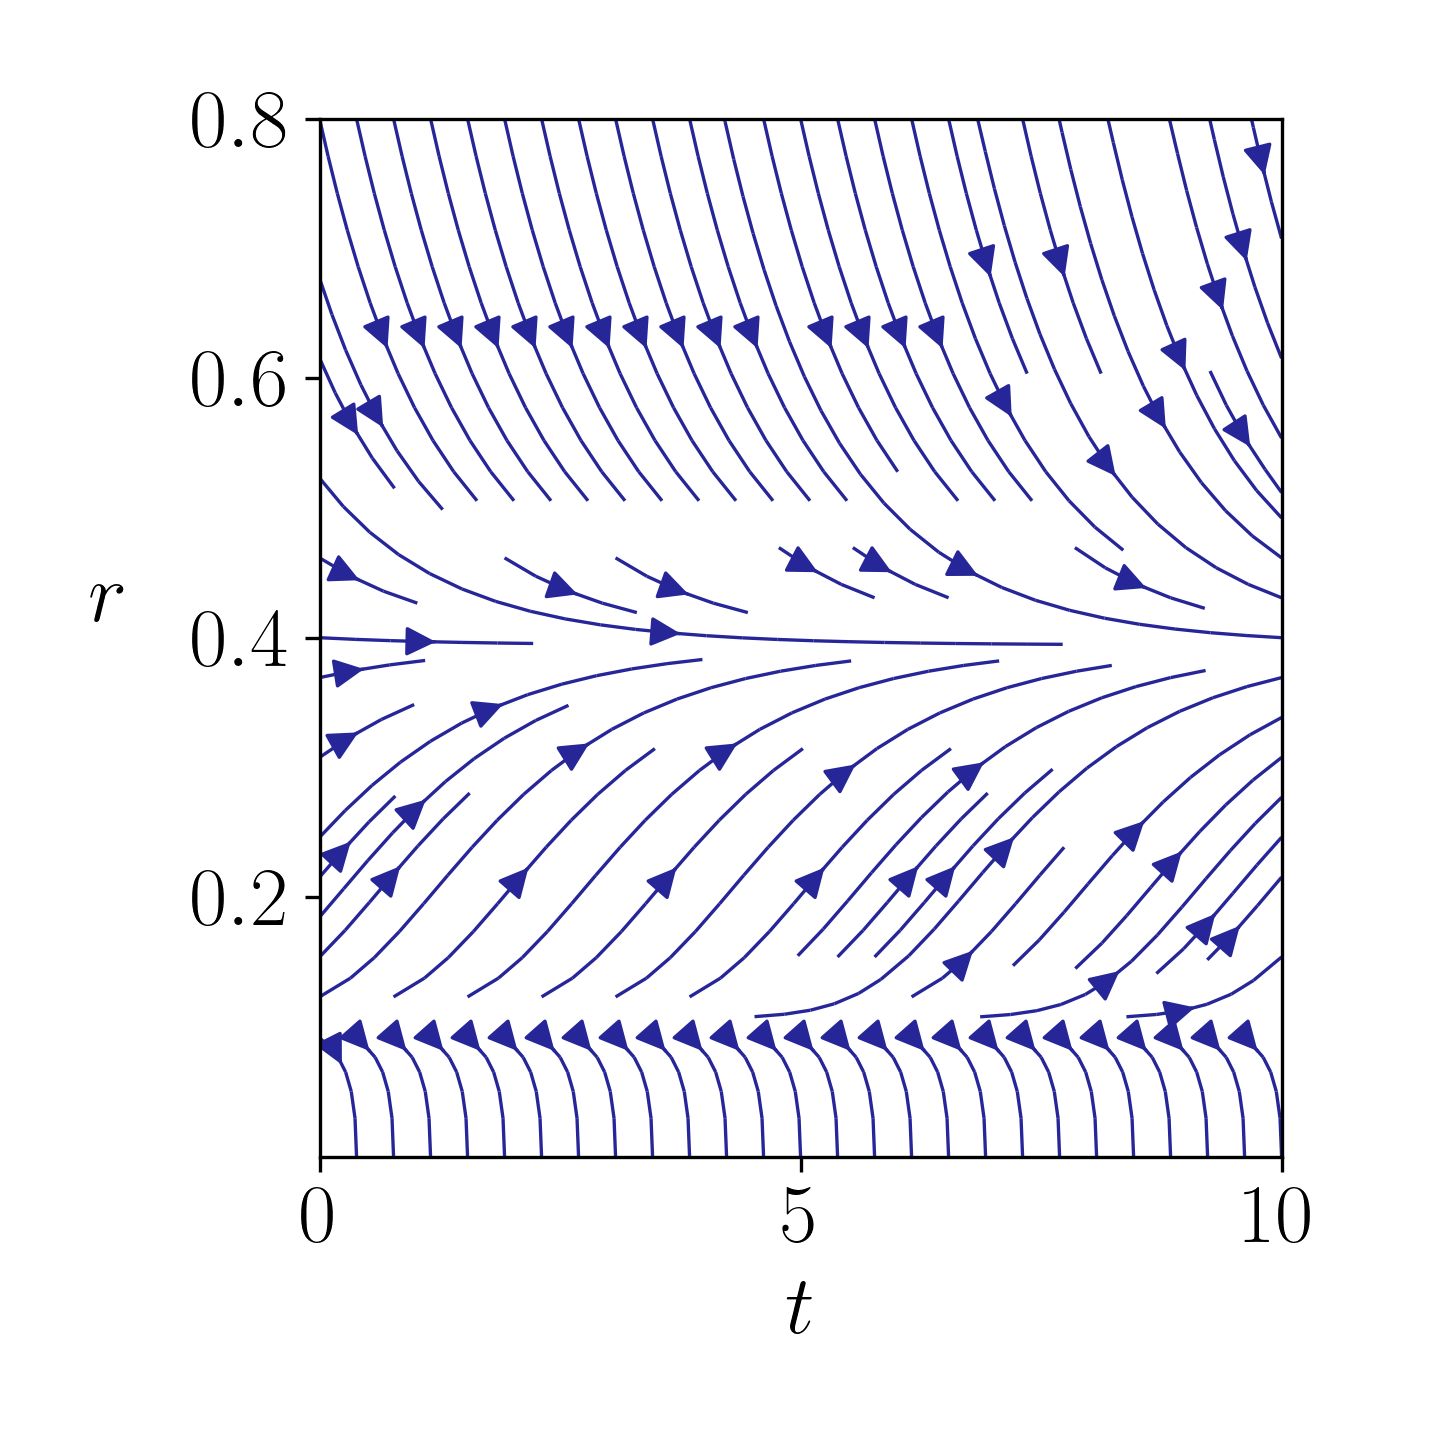
\includegraphics[width=\linewidth]{figures/streamlines/mod1-a96.png}
        \caption{$\alpha=0.96$} 
        \label{fig:radius-characteristics-96} 
    \end{subfigure}
    \begin{subfigure}[b]{0.48\linewidth}
    \centering
        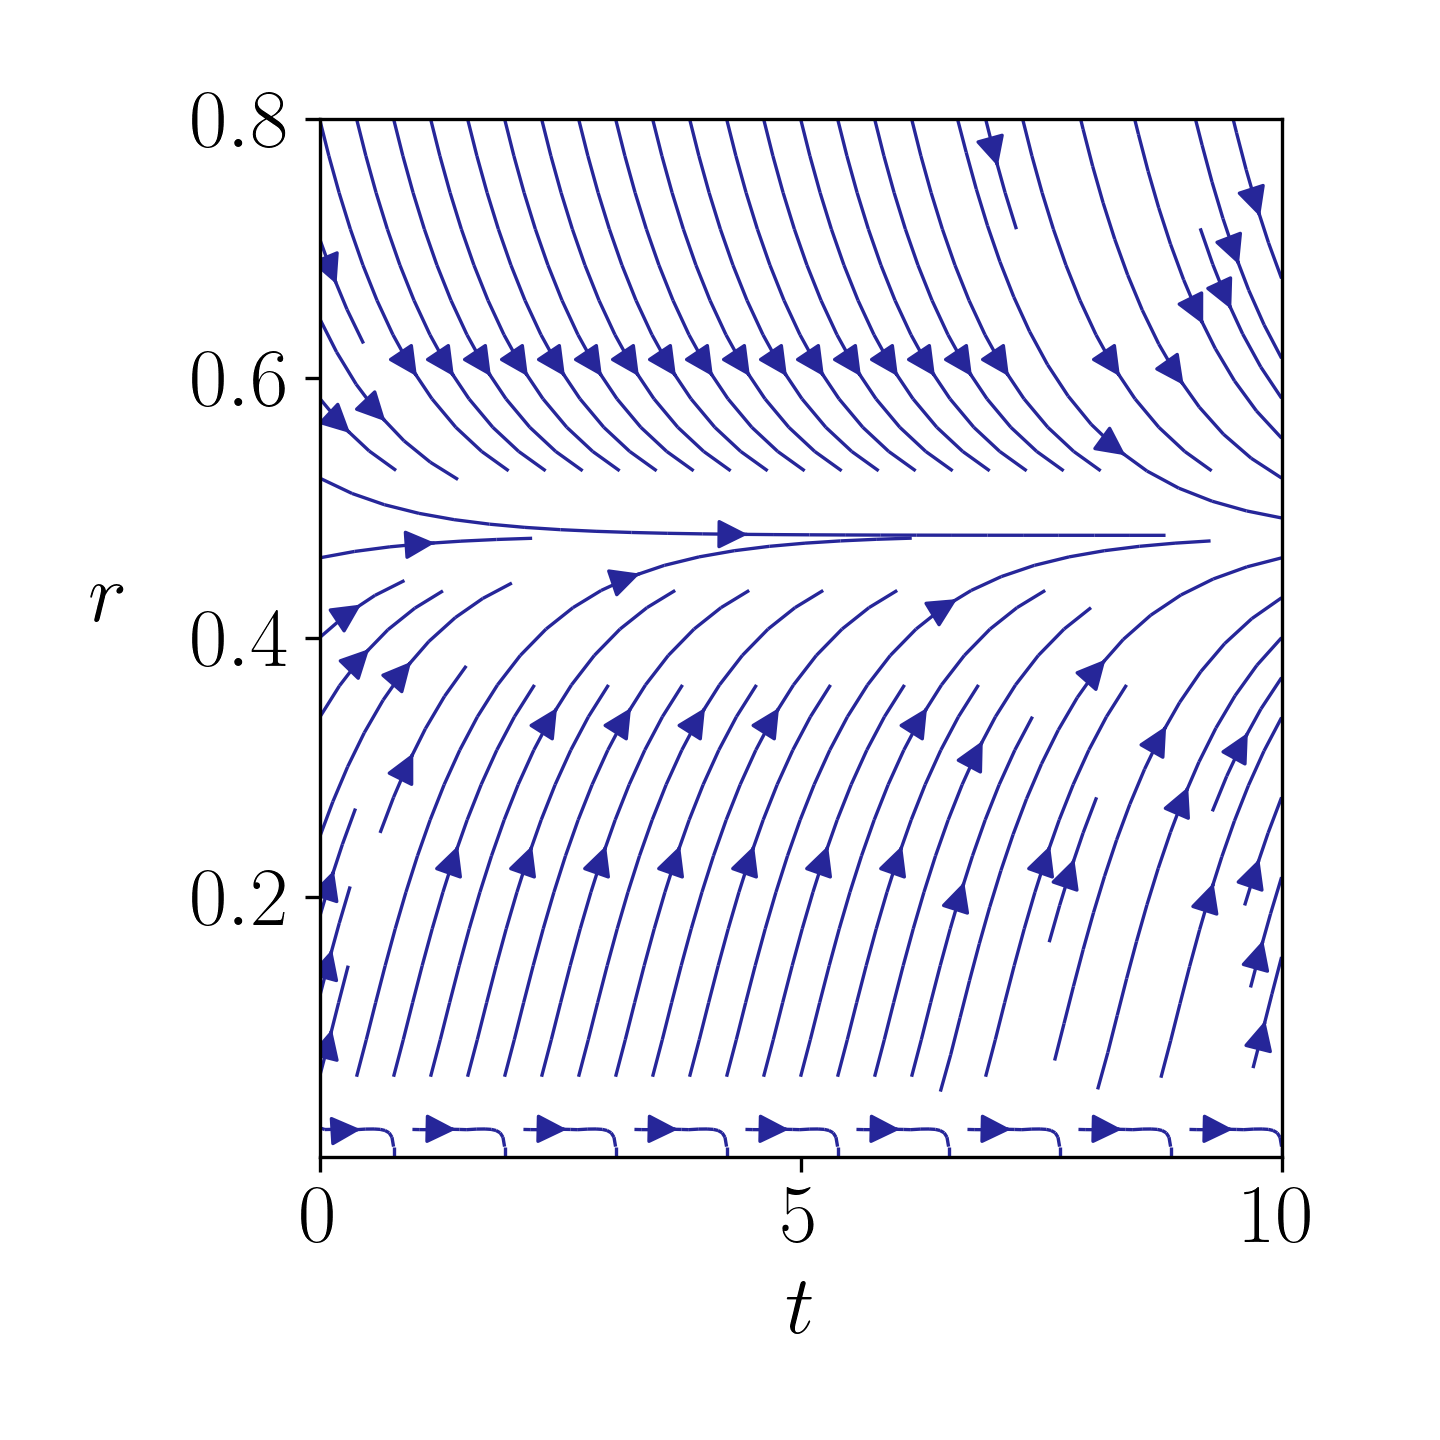
\includegraphics[width=\linewidth]{figures/streamlines/mod1-a99.png}
        \caption{$\alpha=0.99$} 
        \label{fig:radius-characteristics-99} 
    \end{subfigure} 
    \caption[Streamlines in the radially symmetric situation]{Streamlines for the zero level set curve, $\Gamma(t)$, in the radially symmetric situation with the pointset, \pointset, situated at $r_v=0.5$.}
    \label{fig:radius-characteristics}
\end{figure}

The motion of the streamlines can also be viewed in \figref{fig:radius-characteristics}, where we can follow the radius of the zero level set curves starting at a given radius, $r_0$.

We can also construct a general characteristic field for a situation with a fixed $\alpha$, point set radius $r_v$ and initial radius, $r_0$ by solving \eqref{eq:pde-streamline}. First we look at the term $\sigma(t) d(r)$ given the radius of the zero level set curve $r_{\Gamma}$
\begin{alignat}{3}
    \sigma(r_{\Gamma}, t)d(r) &= &|r-r_v| \qquad & \text{when }\radgammam \geq r_v \label{eq:sigma-radius-1}\\
    \sigma(r_{\Gamma}, t)d(r) &= -&|r-r_v| \qquad & \text{when }\radgammam < r_v \label{eq:sigma-radius-2}
\end{alignat}
Thus we can write \eqref{eq:pde-streamline} in terms of $r_\Gamma$ as
\begin{alignat}{3}
    r_t &= -&\bigg(\alpha |r(t)-r_v| + \frac{1-\alpha}{r(t)}\bigg) \qquad &\text{when }\radgammam \geq r_v \\
    r_t &= &\bigg(\alpha |r(t)-r_v| -  \frac{1-\alpha}{r(t)}\bigg) \qquad &\text{when }\radgammam < r_v,
\end{alignat}
Thus, the only thing we need in order to make the full characteristic field is to find the time when $r_{\Gamma} = r_v$, which can be found from \eqref{eq:streamline-solution} and \eqref{eq:streamline-solution-constant}.

This is done in \figref{fig:total-streamline-picture} for a curve starting with $r_0=0.6$ with a point set, $\mathcal{V}$, situated in $r_v=0.5$ and the weighting $\alpha = 0.96$. A useful formula when $(4-\alpha(r_v^2+4))<0$, which is also true for this case, is that the arctangent of an imaginary number is
\begin{equation*}
    \tan^{-1}(i x ) = \frac{i}{2} \ln\bigg(\frac{1+x}{1-x} \bigg).
\end{equation*}

In the figure, we see that the streamlines stemming from the area around the initial curve moves similarily to the zero iso-contours in \figref{fig:radius-characteristics-96}, but further away, they differ more and more. That is because the sign change of $\sigma(r, t)$ happens more and more out of sync with when that particular level set falls into the point set. 

We also observe in the \figref{fig:total-streamline-picture} that level curves in a band around the zero level curve approaches the stationary radius as well. When numerous level curves approach the same radius, the higher dimensional function becomes steeper and steeper. This can cause problems for a numerical scheme which is sensitive to steep gradients.


\begin{figure}
    \begin{subfigure}{.5\linewidth}
        \centering
        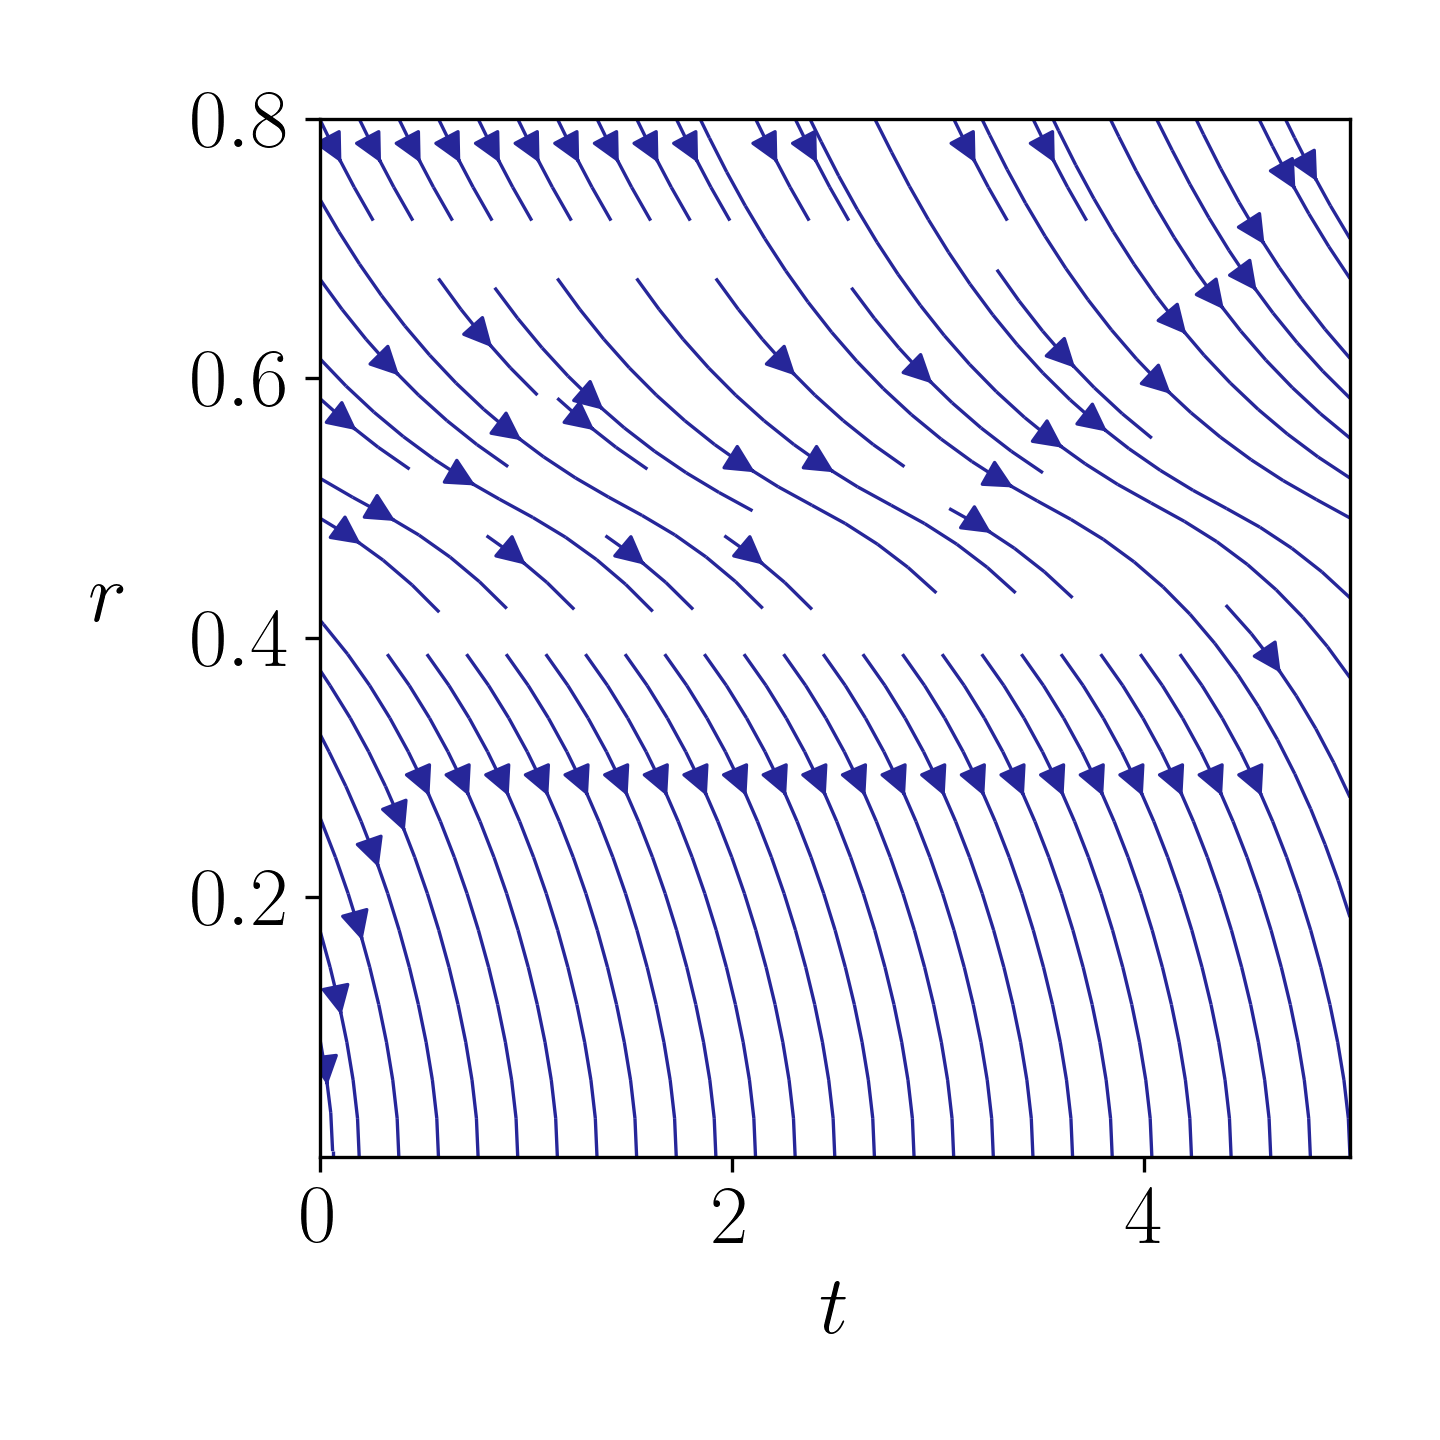
\includegraphics[width=\linewidth]{figures/streamlines/mod1-a96-pos.png}
        \caption{Streamlines with $\sigma(r, t) = 1$}
        \label{fig:sub1}
        \end{subfigure}%
    \begin{subfigure}{.5\linewidth}
        \centering
        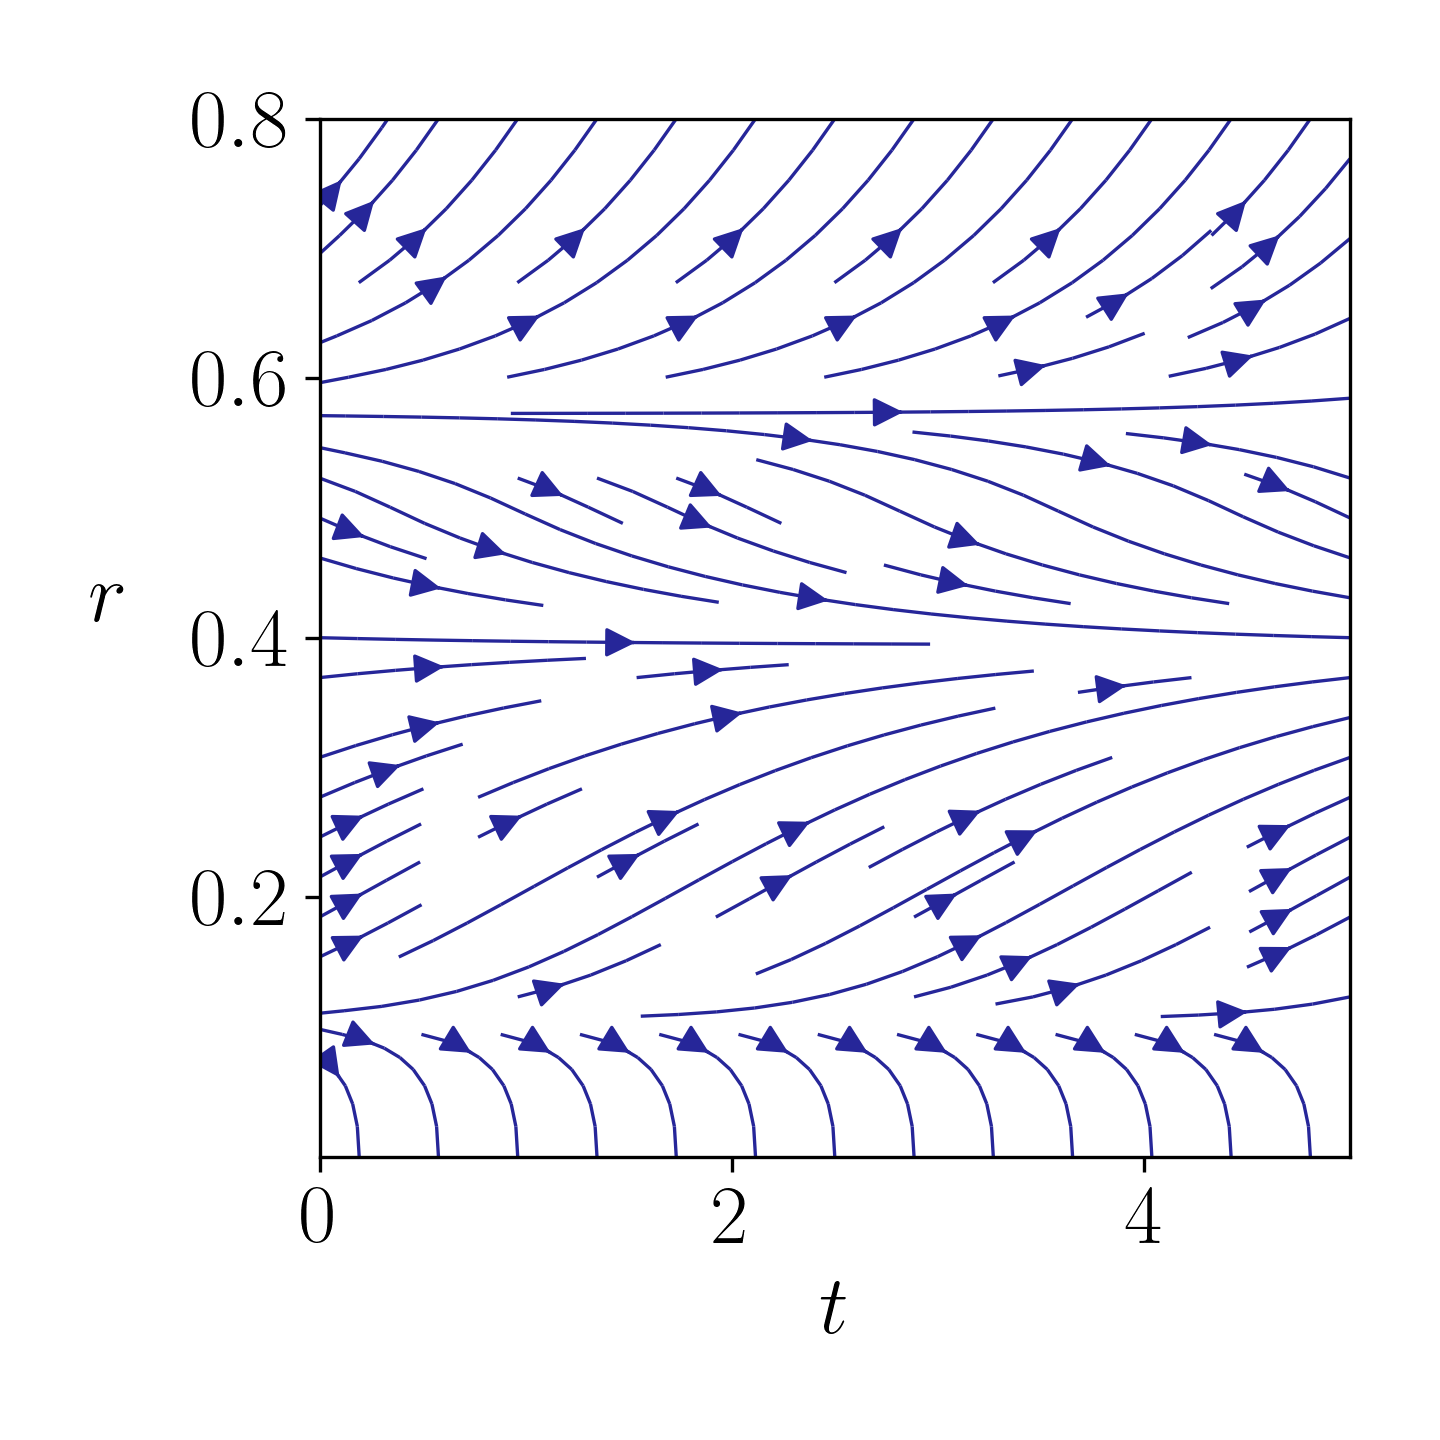
\includegraphics[width=\linewidth]{figures/streamlines/mod1-a96-neg.png}
        \caption{Streamlines when $\sigma(r, t)=-1$}
        \label{fig:sub2}
        \end{subfigure}\\[1ex]
    \begin{subfigure}{\linewidth}
        \centering
        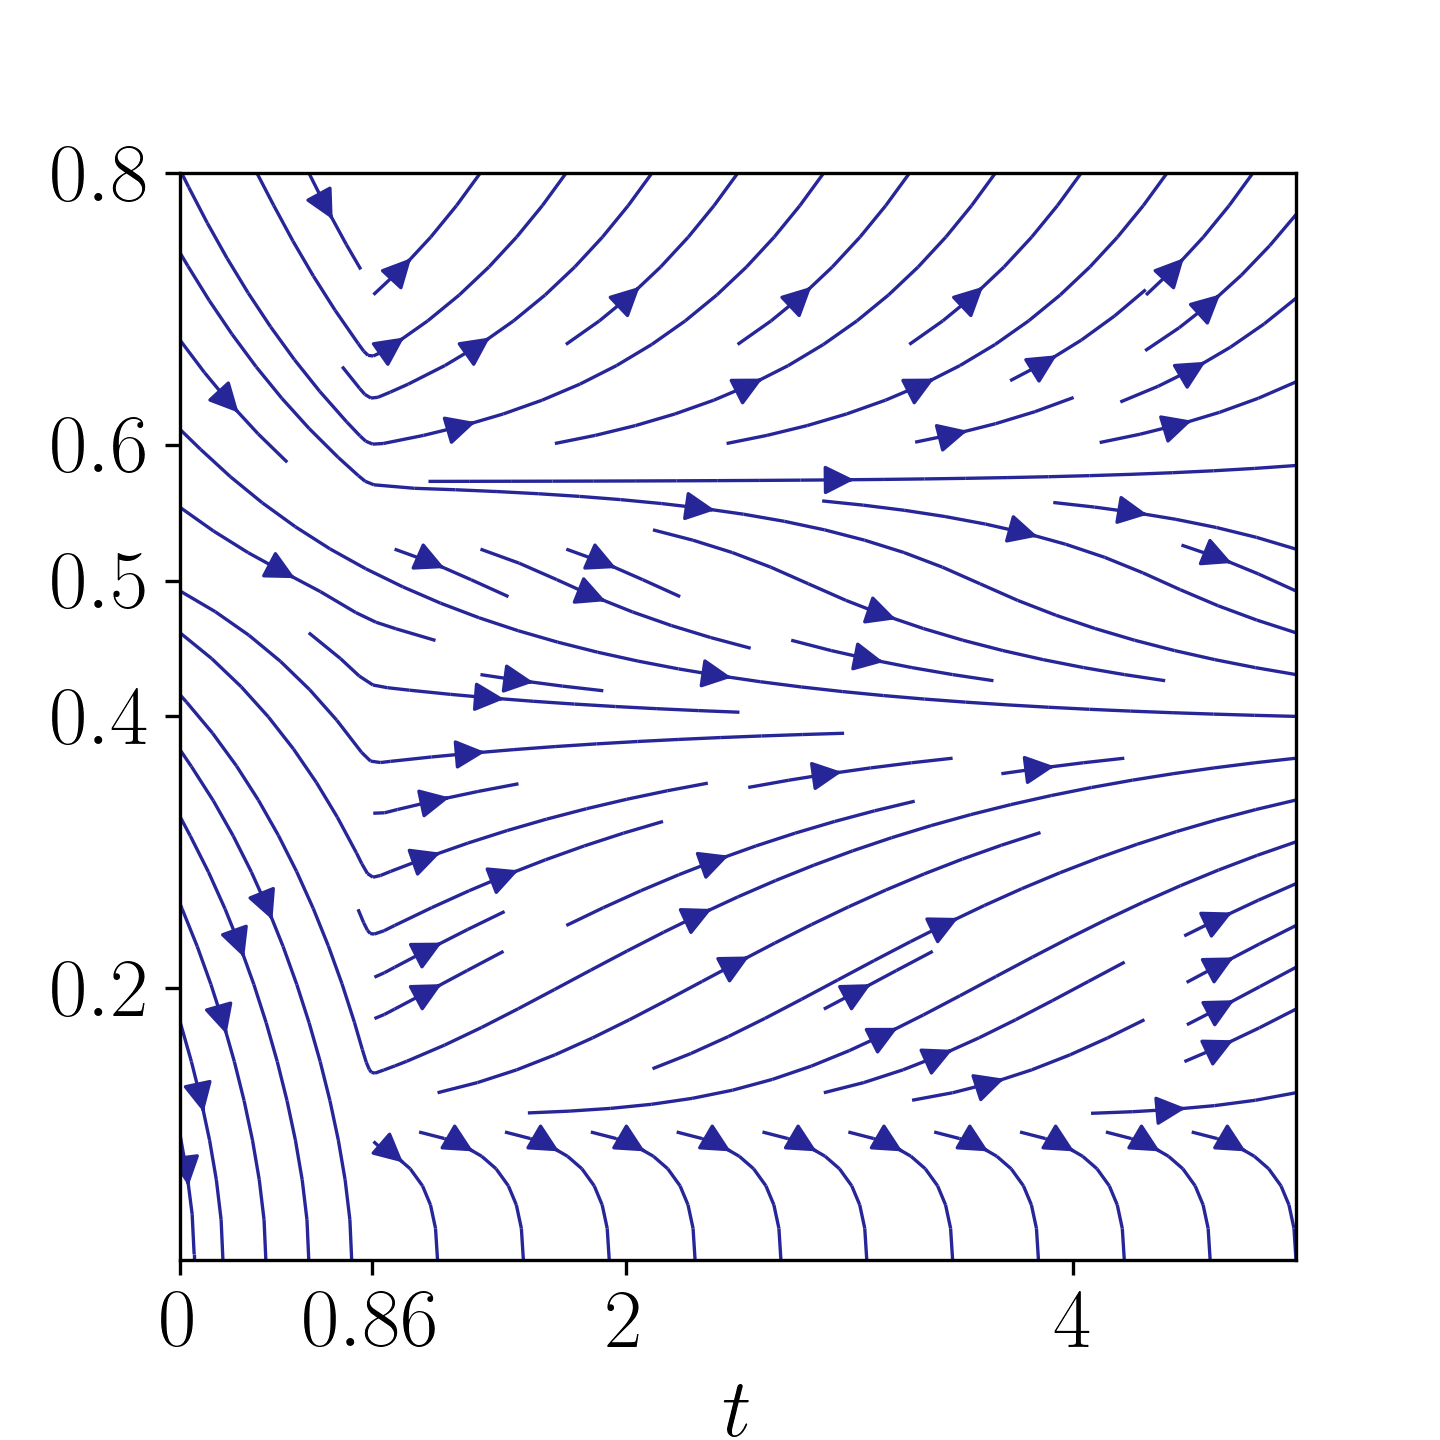
\includegraphics[width=.5\linewidth]{figures/streamlines/mod1-a96-tot.png}
        \caption{Streamlines for all level curves when the zero level set curve, $\Gamma (t)$ has initial radius, $r_0=0.6$.}
        \label{fig:sub3}
    \end{subfigure}
    \caption[Streamlines for all level curves]{Streamlines when the sign function is $\sigma(r, t) = +1$ and $\sigma(r, t) = -1$, for a point set with radius, $r_v=0.5$ and weight $\alpha=0.96$ on top. The lowermost figure shows the streamlines when the zero level set curve has initial radius $r_0=0.6$. Meaning that the sign of $\sigma(r, t)$ changes in $t=0.86$.}
    \label{fig:total-streamline-picture}
\end{figure}

